

\StartOf{Lecture 7}

\Today{(0) Complex Baseband (1) OQPSK  (2) FSK}

\announcements{
\begin{itemize}
  \item For today: Proakis \& Salehi FSK section,   Rice 5.4, 5.5.
  \item Proj 1 due today.  HW 3 due Wed. Proj 2 due one week from today.  
  \item My Office hours: Today 2:30pm-4pm, Tue 11-noon. Keren Li office hour: Wed 4-5 (in Green Hall 2120A).
\end{itemize}
}

\subsection{Complex Baseband for QAM}

First, a short review.  Last lecture, we described QAM and PSK by their use of two basis functions at the same frequency $\omega_0$:
\begin{eqnarray}
  \phi_0(t) &=& \sqrt{2} p(t) \cos(\omega_0 t) \nnn
  \phi_1(t) &=& -\sqrt{2} p(t) \sin(\omega_0 t) \nn
\end{eqnarray}
We outlined the proof that these two are orthogonal.  We looked at some example symbol constellations and calculated their average symbol energies.  We showed that the bandwidth is a function of the pulse shape, for example, for SRRC pulse shapes, $B=(1+\alpha)/T_s$.

Our continuous-time signal will be a sequence of amplitude-scaled versions of these bases:
\begin{equation} \label{E:signal_QAM}
 s(t) = \sqrt{2} \sum_n \left[ a_0(n) p(t-nT_s) \cos(\omega_0 t) - a_1(n)  p(t-nT_s) \sin(\omega_0 t) \right],
\end{equation}
where $a_k(n)$ is the amplitude of $\phi_0$ used during the $n$th symbol period.  We often use $I(t)$, \ie, the in-phase component, as the part of the signal multiplying the $\cos(\omega_0 t)$, and $Q(t)$, \ie, the quadrature component, as the part of the signal multiplying the $\sin(\omega_0 t)$:
\begin{eqnarray}
 && I(t) = \sum_n a_0(n)p(t-nT_s), \quad Q(t) = \sum_n a_1(n)p(t-nT_s).\nnn
 && s(t) = \sqrt{2}  I(t) \cos(\omega_0 t)  - \sqrt{2}  Q(t) \sin(\omega_0 t). \nn
\end{eqnarray}
Alternatively, 
\begin{equation} \label{E:signal_Angle}
 s(t) = \sqrt{2} \sum_n \sqrt{a_0^2(n) + a_1^2(n)} p(t-nT_s) \cos\left(\omega_0 t + \tan^{-1} \frac{a_1(n)}{a_0(n)} \right) ,
\end{equation}
a form that shows that $s(t)$ during any symbol has an ``envelope'' or amplitude and a phase angle.  The envelope and angle are time-varying functions because the pulse amplitude is not constant.  

When we plot the in-phase vs. the quadrature, Rice calls it the ``phase trajectory plot''.  Actually, it shows the trajectory of both the phase and envelope.  An example for QPSK is shown in  Figure \ref{F:SimulationQPSK}.

\begin{figure}[htbp]
$\begin{array}{ll}
  (a)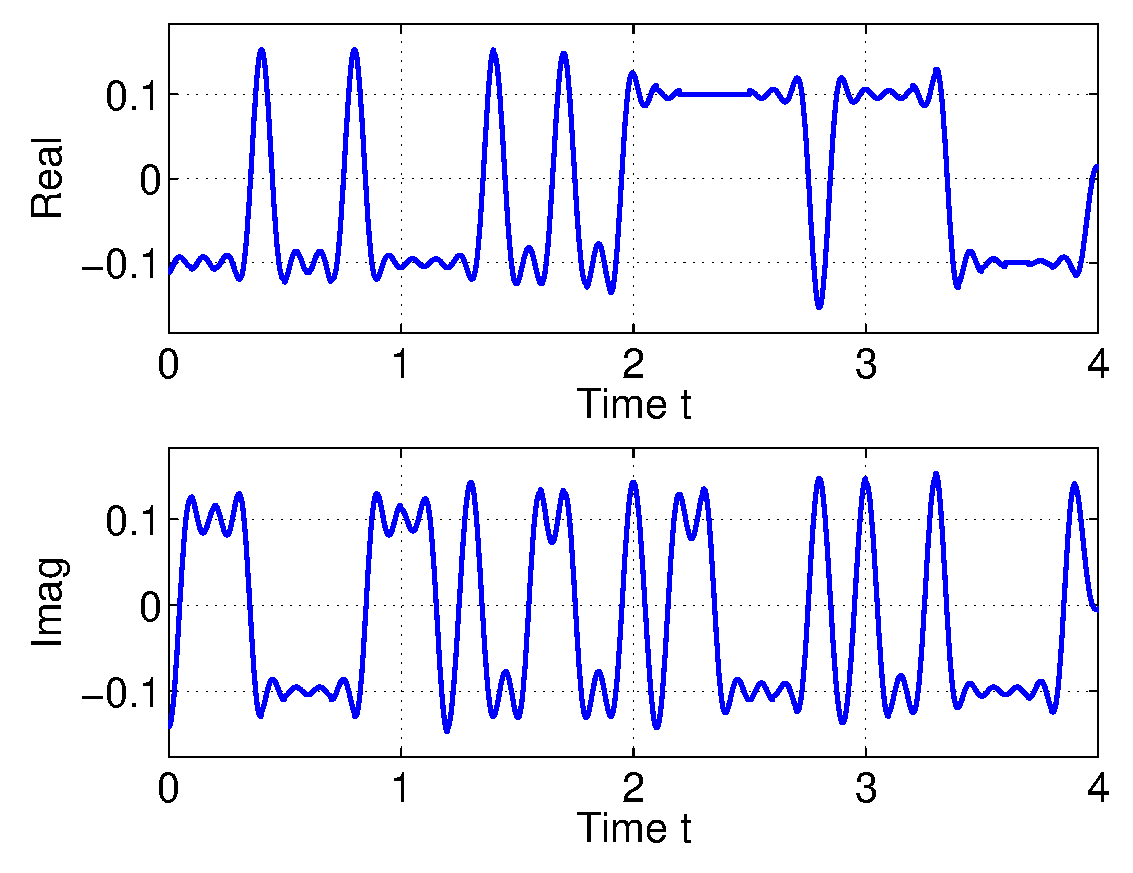
\includegraphics[width=0.45\textwidth]{../images/plotComplexSigQPSK.eps} &
  (b)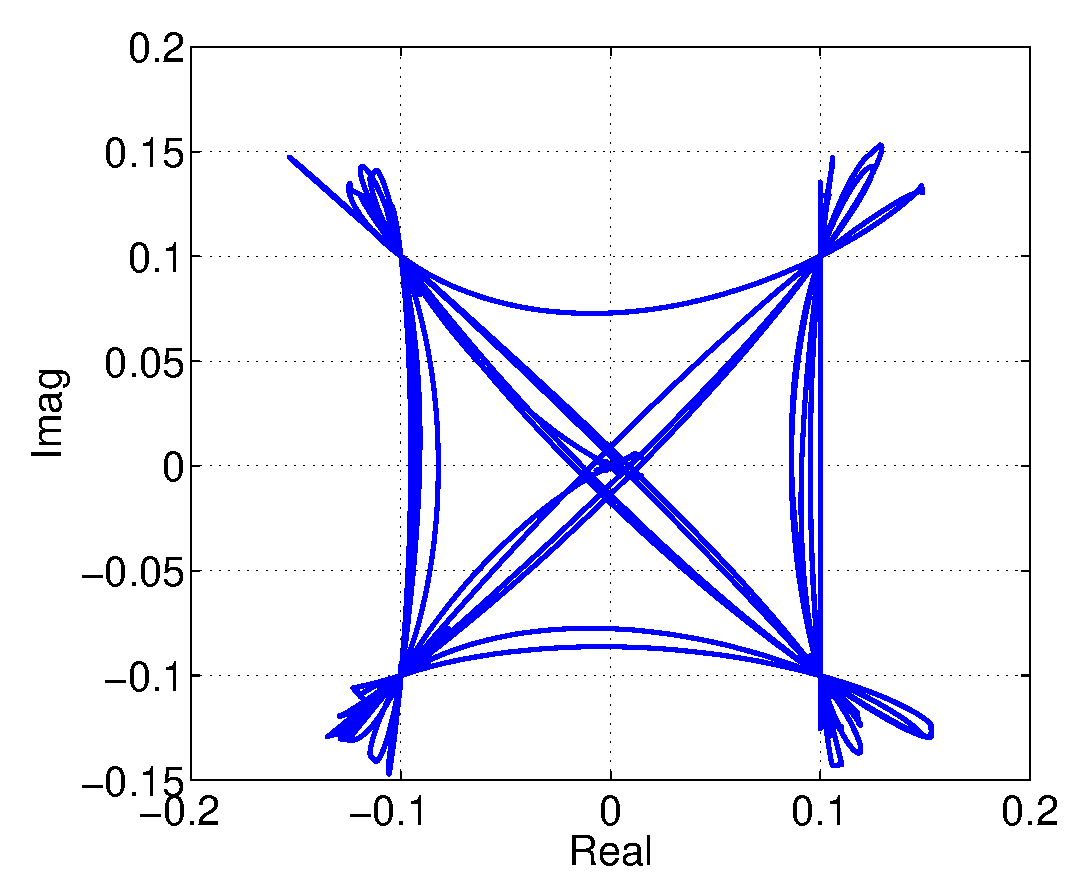
\includegraphics[width=0.45\textwidth]{../images/plotConstellationDiagramQPSK.eps}\\
  \end{array}$
  \caption{Matlab simulation of the complex baseband form of $s(t)$ for QPSK, showing the (a) in-phase (cosine) and quadrature (sine) components.  In the phase trajectory plot in (b), time is removed and we plot the in-phase vs.~the quadrature components.}
  \label{F:SimulationQPSK}
\end{figure}



\section{Offset QPSK (OQPSK)}

\subsection{Motivation}

One thing that makes a transmitter more power hungry is the need for a linear amplifier.  An amplifier uses DC power to take a bandpass input signal and increase its
amplitude at the output.  If $P_{DC}$ is the input power (\eg, from
battery) to the amplifier, and $P_{out}$ is the output signal power,
the power efficiency is rated as $\eta_P = P_{out} / P_{DC}$.

Truly linear amplifiers (class A) amplifiers are at most 50\% power efficient.  We are interested in the question, what signals can be amplified with nonlinear (class C) amplifiers that are around 90\% power efficient?  The answer is that ``constant envelope'' signals can.  These are signals that the peak envelope is never much higher than the average envelope.  The phase trajectory plot of a constant envelope signal will be nearly a circle, and it will never go through or near the origin (envelope of zero).

Not all modulations are constant envelope, so this involves some modulation limitations. In order to double the power efficiency, battery-powered transmitters are often willing to use constant envelope modulations so that they can use Class C amplifiers.  They can
do this if their output signal has constant envelope.  

\subsection{Definition}

The reason that QPSK is not constant envelope is that when the phase angle changes 180 degrees from one symbol to the next, the envelope will go through zero.  See Figure \ref{F:SimulationQPSK} to see this graphically.

Offset QPSK solves this problem by simply shifting one of the basis functions forward by half a symbol period, \ie, $T_s/2$.  The orthonormal basis for OQPSK are thus:
\begin{eqnarray}
  \phi_0(t) &=& \sqrt{2} p(t) \cos(\omega_0 t) \nnn
  \phi_1(t) &=& \sqrt{2} p(t - T_s/2) \sin(\omega_0 t) \nn
\end{eqnarray}
We still only offset subsequent symbols by $T_s$, so the transmitted signal is:
\[
 s(t) = \sqrt{2} \sum_n \left[ a_0(n) p(t-nT_s) \cos(\omega_0 t) + a_1(n)  p\left(t-\left(n+\frac{1}{2}\right)T_s\right) \sin(\omega_0 t) \right],
\]
or equivalently the in-phase and quadrature components are,
\[
 I(t) = \sqrt{2} \sum_n a_0(n)p(t-nT_s), \quad Q(t) = \sqrt{2} \sum_n a_1(n)p\left(t-\left(n+\frac{1}{2}\right)T_s\right).
\]
Compared to (\ref{E:signal_QAM}), the in-phase component of $s(t)$ in OQPSK does not go through zero at the same times that the quadrature component does, since the pulse functions $p()$ are offset in time by half a symbol period.  

Another way to look at this is to view the phase trajectory plot in Figure \ref{F:SimulationOQPSK}.  The signal never switches from its current constellation point to the one 180$^o$ opposite -- either the in-phase or quadrature component changes during any multiple of $T_s/2$, but NOT both.

\begin{figure}[htbp]
$\begin{array}{ll}
  (a)\includegraphics[width=0.45\textwidth]{../images/plotComplexSigOQPSK.eps} &
  (b)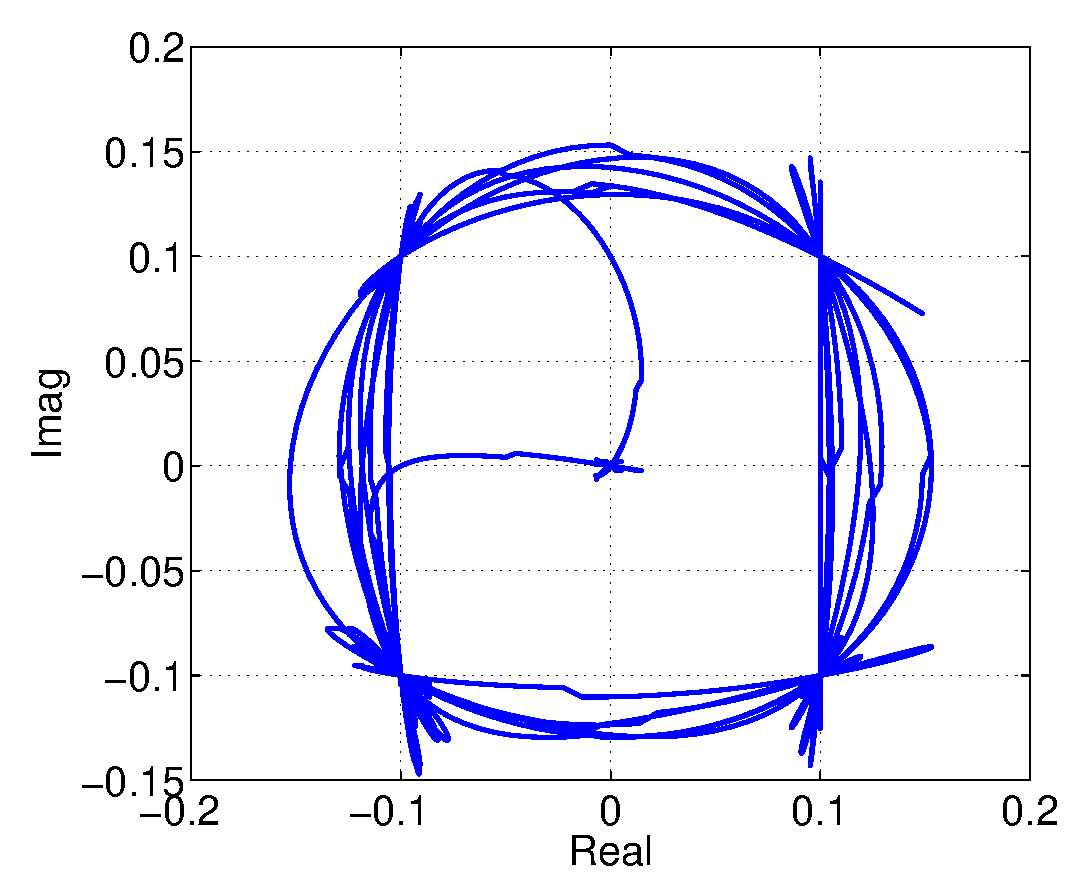
\includegraphics[width=0.45\textwidth]{../images/plotConstellationDiagramOQPSK.eps}
  \end{array}$
  \caption{Matlab simulation of $s(t)$ for OQPSK, showing the (a) in-phase (cosine) and quadrature (sine) components.  The phase trajectory plot in (b) shows the nearly constant envelope of OQPSK, compared to that for QPSK in Figure \ref{F:SimulationQPSK}.}
  \label{F:SimulationOQPSK}
\end{figure}


At the receiver, we just need to delay the sampling on the
in-phase component of the signal half of a sample period with respect to the quadrature
signal.  The new transmitted signal takes the same bandwidth and
average power, and as we will show later in the course, the same $E_b/N_0$ vs.~probability of bit
error performance.  However, the envelope $|s(t)|$ is largely
constant.  Compare Figures \ref{F:SimulationQPSK} and \ref{F:SimulationOQPSK} to see the differences between QPSK and OQPSK.

\section{Frequency Shift Keying (FSK)}

In frequency shift keying, symbols are selected to be sinusoids
with frequency selected among a set of $M$ different frequencies
$\{f_0, f_1, \ldots f_{M-1}\}$.  Note that in FSK, the number of basis functions equals the number of symbols.  Consider $f_{k} = f_c + k\Delta f$, and thus
\begin{equation} \label{E:FSK-Symbols4}
 \phi_k(t) = \sqrt{2} p(t) \cos(\omega_0 t + 2\pi k\Delta f t)
\end{equation}
where $p(t)$ is our pulse shape.  We want these $\phi_k(t)$ to form an orthonormal basis.  How can we make them orthonormal?  First, note that these basis functions are unit energy, just like we've shown that the QAM basis functions are unit energy.  Next, what do we get when we find the inner product of two different basis functions,  $\phi_k(t)$ and $\phi_m(t)$ for $m\neq k$?

\begin{eqnarray}
 \langle \phi_k(t), \phi_m(t) \rangle &=&  \int_{t=0}^{T_s} (2/T_{s}) \cos(\omega_0 t + 2\pi k\Delta f t)  \cos(\omega_0 t + 2\pi m\Delta f t) dt
     \nonumber \\
   &=& 1/T_{s} \int_{t=0}^{T_{s}} \cos(2\pi (k-m)\Delta f t) dt +
   \nonumber \\
   & & 1/T_{s} \int_{t=0}^{T_{s}} \cos(2 \omega_0 t + 2\pi (k+m)\Delta f  t) dt
     \nonumber \\
   &=& 1/T_{s} \left[ \frac{\sin(2\pi (k-m)\Delta f t)}{2\pi (k-m)\Delta f } \right|_{t=0}^{T_{s}}
     \nonumber \\
   &=&  \frac{\sin(2\pi (k-m)\Delta f T_{s})}{2\pi (k-m)\Delta f T_{s}}
     \nonumber
\end{eqnarray}

Yes, they are orthogonal if $2\pi (k-m)\Delta f T_{s}$ is a multiple
of $\pi$.  (They are also approximately orthogonal if $\Delta f$ is really big, but we don't want to waste spectrum.) For general $k\ne m$, this requires that $\Delta f T_{s}
= n/2$, \ie,
\begin{equation} \label{E:Delta_f_FSK}
  \Delta f = n \frac{1}{2T_{s}} = n \frac{f_{s}}{2}
\end{equation}
for integer $n$. (Otherwise, no they're not.)

Thus we need to plug into (\ref{E:FSK-Symbols4}) for $\Delta f = n
\frac{1}{2T_{s}}$ for some integer $n$ in order to have an
orthonormal basis.  What $n$?  In practice, we either use an $n$
of 1 or 2. Using $n=1$ is called \emph{minimum shift keying} (MSK) since it is the minimum frequency spacing.  Use of $n=2$ is historically more common because it can be implemented with a non-coherent receiver, as we discuss below.

Signal space vectors $\mba_i$ are given by
\begin{eqnarray}
  \mba_0 &=& [A, 0, \ldots, 0] \nonumber \\
  \mba_1 &=& [0, A, \ldots, 0] \nonumber \\
  &\vdots & \nonumber \\
  \mba_{M-1} &=& [0, 0, \ldots, A] \nonumber
\end{eqnarray}
What is the average energy per symbol?  This means that $A =
\sqrt{\En_s}$.

For $M=2$ and $M=3$ these vectors are plotted in Figure \ref{F:FSK-signalSpaceDiagram}.

\begin{figure}[htbp]
  \centerline{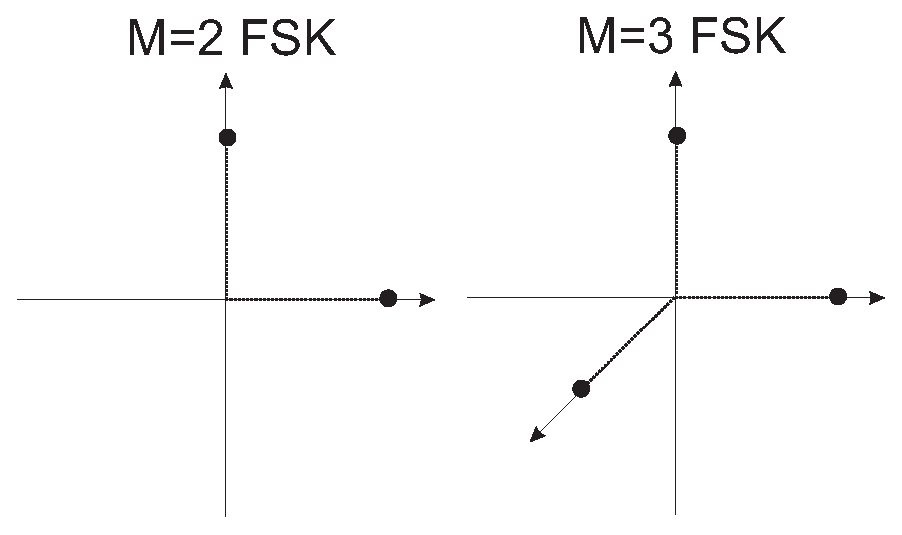
\includegraphics[width=0.4\textwidth]{../images/FSK-signalSpaceDiagram.eps}}
  \caption{Signal space diagram for $M=2$ and $M=3$ FSK modulation.}
  \label{F:FSK-signalSpaceDiagram}
\end{figure}


\subsection{Transmission of FSK}

FSK can be seen as a sum of $M$ different carrier signals, each multiplied by a pulse shape $p(t)$.  In practice, FSK signals are usually generated from a single VCO, as seen in Figure
\ref{F:FSK-TX-BlockDiagram}.

\Definition{Voltage Controlled Oscillator (VCO)}{A sinusoidal
generator with frequency that linearly proportional to an input
voltage.}

Note that we don't need to (and don't want to) send square wave input into the VCO.  The transition can be set to smoothly switch from one frequency to the next.

\Definition{Continuous Phase Frequency Shift Keying (CPFSK)}{FSK with no
phase discontinuity between symbols.  In other words, the phase of
the output signal $\phi_k(t)$ does not change instantaneously at
symbol boundaries $iT_{s}$ for integer $i$, and thus $\phi(t^- +
iT_{s}) = \phi(t^+ + iT_{s})$ where $t^-$ and $t^+$ are the
limiting times just to the left and to the right of 0,
respectively.}

There are a variety of flavors of CPFSK, which are beyond the scope of this course.

\begin{figure}[htbp]
  \centerline{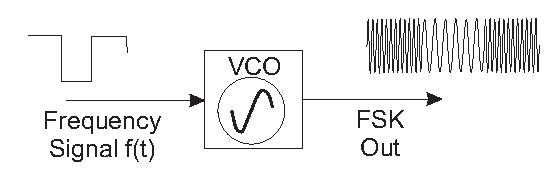
\includegraphics[width=0.6\textwidth]{../images/FSK-BlockDiagram.eps}}
  \caption{Block diagram of a binary FSK transmitter.}
  \label{F:FSK-TX-BlockDiagram}
\end{figure}

\subsection{Reception of FSK}

FSK reception is either phase coherent or phase non-coherent.  Here,
there are $M$ possible carrier frequencies, so we'd need to know and
be synchronized to $M$ different phases $\theta_i$, one for each
symbol frequency:
\begin{eqnarray}
  && \cos(\omega_0 t  + \theta_0)
    \nonumber \\
  && \cos(\omega_0 t  + 2\pi \Delta f t + \theta_1)
    \nonumber \\
    &  & \vdots \nonumber \\
  && \cos(\omega_0 t + 2\pi (M-1)\Delta f t + \theta_{M-1})
    \nonumber
\end{eqnarray}

\subsection{Coherent Reception}

FSK reception can be done via a correlation receiver, just as we've
seen for previous modulation types.

Each phase $\theta_k$ is estimated to be $\hat{\theta}_k$ by a
separate phase-locked loop (PLL). In one flavor of CPFSK (called Sunde's FSK), the carrier $\cos(2\pi f_k t + \theta_k)$ is sent with
the transmitted signal, to aid in demodulation (at the expense of
the additional energy).  This is the only case where I've heard of
using coherent FSK reception.

As $M$ gets high, coherent detection becomes difficult.  These $M$
PLLs must operate even though they can only synchronize when their
symbol is sent, $1/M$ of the time (assuming equally-probable
symbols). Also, having $M$ PLLs is a drawback.


\subsection{Non-coherent Reception}

Notice that in Figure \ref{F:FSK-signalSpaceDiagram}, the sign or
phase of the sinusoid is not very important -- only one symbol
exists in each dimension.  In non-coherent reception, we just
measure the energy in each frequency.

This is more difficult than it sounds, though -- we have a
fundamental problem. As we know, for every frequency, there are two
orthogonal functions, cosine and sine (see QAM and PSK).  Since we
will not know the phase of the received signal, we don't know
whether or not the energy at frequency $f_{k}$ correlates highly with
the cosine wave or with the sine wave.  If we only correlate it with
one (the sine wave, for example), and the phase makes the signal the
other (a cosine wave) we would get a inner product of zero!

The solution is that we need to correlate the received signal with
both a sine and a cosine wave at the frequency $f_{k}$.  This will
give us two inner products, lets call them $x_{k}^I$ using the
capital $I$ to denote in-phase and $x_{k}^Q$ with $Q$ denoting
quadrature.

\begin{figure}[htbp]
  \centerline{\includegraphics[width=0.45\textwidth]{../images/FSK_Energy_Diagram.eps}}
  \caption{The energy in a non-coherent FSK receiver at one frequency $f_k$ is calculated by
  finding its correlation with the cosine wave ($x_{k}^I$) and sine wave ($x_{k}^Q$) at the frequency of interest, $f_{k}$, and
  calculating the squared length of the vector $[x_{k}^I, x_{k}^Q]^T$.}
  \label{F:FSK_Energy_Diagram}
\end{figure}

The energy at frequency $f_{k}$, that is,
\[
 \En_{f_{k}} =  (x_{k}^I)^2 +  (x_{k}^Q)^2
\]
is calculated for each frequency $f_{k}$, $k=0, 1, \ldots, M-1$, and the detector picks the $k$ that maximizes $\En_{f_{k}}$.  

However, energy detection works only when $n=2$ in (\ref{E:Delta_f_FSK}).  (Showing this might be a good homework or exam problem.)  That is, $\Delta f = 1/T_s$.  Some FSK systems trade off the extra bandwidth usage in order to allow for a less complicated receiver design (an energy detector).

\subsection{Bandwidth of FSK}

Carson's rule is used to calculate the bandwidth of FM signals.  For
$M$-ary FSK, it tells us that the approximate bandwidth is,
\[
B_{M-FSK} = (M-1) \Delta f + B_{p(t)}
\]
where $B_{p(t)}$ is the two-sided bandwidth of the pulse shape.
For root raised-cosine pulse shaping, the null-to-null bandwidth is 
$B_{p(t)}=(1+\alpha)/T_s$. 

